\documentclass[a4paper, 12pt]{scrartcl}
\usepackage[sexy]{evan}
\usepackage{amsmath,amssymb}
\usepackage[utf8]{inputenc}
\usepackage{xcolor}
\usepackage[paperwidth=16cm, paperheight=16cm,margin=1cm]{geometry}
\usepackage{graphicx}
\usepackage{tikz}
\usepackage{tkz-euclide}
\usetikzlibrary{calc}
\usetikzlibrary{intersections}

\usepackage{array,multirow}
\usetikzlibrary{angles}
\usepackage{adjustbox}
%--------------------------
%-------------------------
\usepackage{systeme}
\usepackage{hyperref}
\usepackage{multicol}
\usepackage[symbol]{footmisc}
\usetikzlibrary{calc}
\pagestyle{empty}
\let \ds \displaystyle
%-------
\newcommand\kunci{%
 \tikz[overlay]\draw[red] (-2ex,.7ex) circle (1.7ex);%
 }
 \newcommand\ralat{%
 \tikz[overlay]\draw[blue] (-2ex,.7ex) circle (1.7ex);%
 }
%-----------
\newcommand{\siku}[4][.21cm]
	{
	\coordinate (tempa) at ($(#3)!#1!(#2)$);
	\coordinate (tempb) at ($(#3)!#1!(#4)$);
	\coordinate (tempc) at ($(tempa)!0.5!(tempb)$);%midpoint
	\draw[black] (tempa) -- ($(#3)!2!(tempc)$) -- (tempb);
	}
	\usetikzlibrary{calc,positioning,intersections} %----------
%-------------------------TRIGON
 \renewcommand{\baselinestretch}{1.3}

\makeatother
%-
\ihead{\footnotesize }
\ohead{\footnotesize }
\title{Piramida Emas Siskacohl}
\author{}
\date{}
\let \ds \displaystyle
\pagestyle{empty}
\let \measureangle \mda
\parindent0cm

\usepackage{pagecolor}% http://ctan.org/pkg/{pagecolor,lipsum}

\newcommand\progtitle[1]{{\vspace{0.2cm}\begin{center}\Large\bfseries #1 \end{center}\vspace{0.2cm}}}

\begin{document}
\progtitle{Satu Soal Banyak Cara\\ - Euclid, Analit, Kompleks, Barycentric}
\section{Soal}
Diberikan segitiga $ABC$ dengan dua persegi $ABPQ$ dan $ACQM$ dikonstruksi ke arah luar $\triangle ABC$. Jika $D$ adalah titik tengah $BC$ dan $DA$ memotong $MN$ di $T$, buktikan bahwa $AT \perp MN$. 

\begin{center}
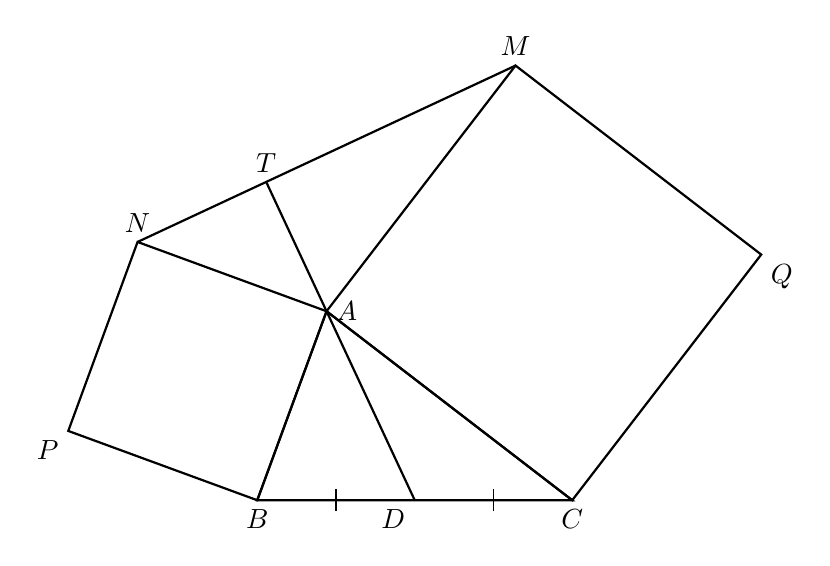
\begin{tikzpicture}[scale=0.8]
       \coordinate[label=right:$A$] (A) at (1.1,3);
       
       \coordinate[label=below: $B$] (B) at (0,0);
       
       \coordinate[label= below:$C$] (C) at (5,0);
       
       \coordinate[label=below left:$D$] (D) at ($(B) !0.5! (C)$);
       
       \tkzMarkSegment[pos=0.5,mark=|](B,D)
       \tkzMarkSegment[pos=0.5,mark=|](C,D)
       
       \coordinate[label=below left:$P$] (P) at ($ (B)!1!90:(A)$);
       \coordinate[label=above:$N$] (N) at ($ (A)!1!-90:(B)$);
       
       \coordinate[label=below right:$Q$] (Q) at ($ (C)!1!-90:(A) $);
       \coordinate[label=above:$M$] (M) at ($ (A)!1!90:(C) $);
       
       \draw[name path=ad, thick] (D) -- (A);
       
       \draw[thick] (A) -- (B) -- (C) -- cycle;
       
       \draw[thick] (A) -- (C) --  (Q) -- (M) -- cycle;
       
       \draw[thick] (A) -- (B) -- (P) -- (N) -- cycle;
       
       \draw[name path=mn, thick] (M) -- (N);
       
       \coordinate[label=above:$T$] (T) at ($(M)!(A)!(N)$);
       \draw[thick] (T) -- (A);
\end{tikzpicture}
\end{center}

\newpage

\section{Solusi Synthetic / Euclid}
\begin{center}
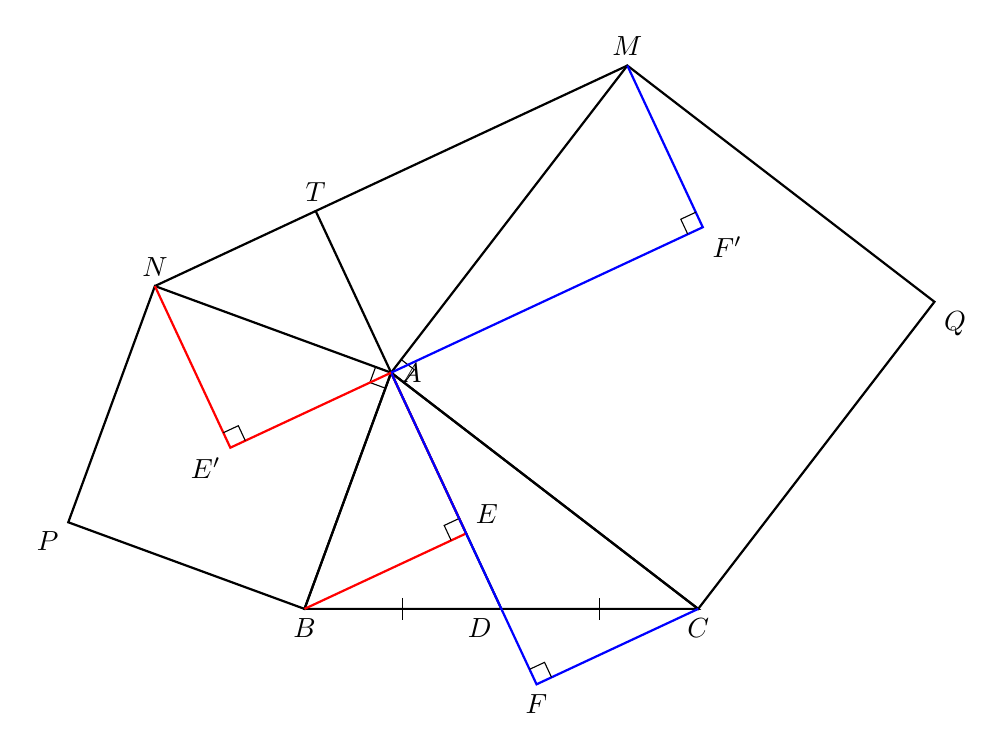
\begin{tikzpicture}
\coordinate[label=right:$A$] (A) at (1.1,3);
       
       \coordinate[label=below: $B$] (B) at (0,0);
       
       \coordinate[label= below:$C$] (C) at (5,0);
       
       \coordinate[label=below left:$D$] (D) at ($(B) !0.5! (C)$);
       
       \tkzMarkSegment[pos=0.5,mark=|](B,D)
       \tkzMarkSegment[pos=0.5,mark=|](C,D)
       
       \coordinate[label=below left:$P$] (P) at ($ (B)!1!90:(A)$);
       \coordinate[label=above:$N$] (N) at ($ (A)!1!-90:(B)$);
       
       \coordinate[label=below right:$Q$] (Q) at ($ (C)!1!-90:(A) $);
       \coordinate[label=above:$M$] (M) at ($ (A)!1!90:(C) $);
       
       \draw[name path=ad, thick] (D) -- (A);
       
       \draw[thick] (A) -- (B) -- (C) -- cycle;
       
       \draw[thick] (A) -- (C) -- (Q) -- (M) -- cycle;
       
       \draw[thick] (A) -- (B) -- (P) -- (N) -- cycle;
       
       \draw[name path=mn, thick] (M) -- (N);
       
       \siku{N}{A}{B}
       \siku{M}{A}{C}
       
       \coordinate[label=above:$T$] (T) at ($(M)!(A)!(N)$);
       \draw[thick] (T) -- (A);
       
       \coordinate[label=above right:$E$] (E) at ($(A)!(B)!(D)$);
       \draw[thick, color=red] (A) -- (E) -- (B);
       \siku{A}{E}{B}
       
       \coordinate[label=below:$F$] (F) at ($(A)!(C)!(D)$);
       \draw[thick, color=blue] (A) -- (F) -- (C);
       \siku{A}{F}{C}
       
       \coordinate[label=below left:$E'$] (E') at ($(A)!1!-90:(E)$);
       \draw[thick, color=red] (N) -- (E') -- (A);
       \siku{A}{E'}{N}
       
       \coordinate[label=below right:$F'$] (F') at ($(A)!1!90:(F)$);
       \draw[thick, color=blue] (M) -- (F') -- (A);
       \siku{A}{F'}{M}
\end{tikzpicture}
\end{center}

Misalkan proyeksi titik $B$ dan $C$ pada garis $AD$ berturut-turut adalah $E$ dan $F$. Perhatikan bahwa $BE \parallel FC$ yang menyebabkan $\triangle BED \sim \triangle CFD$. Namun, karena $BD=DC$, maka $\triangle BED \cong \triangle CFD$ sehingga $BE=FC$. 

Selanjutnya misalkan $E'$ adalah hasil rotasi titik $E$ sejauh $-90^\circ$ terhadap pusat $A$ dan $F'$  adalah hasil rotasi titik $F$ sejauh $90^\circ$ terhadap pusat $A$. Amati dari hasil rotasi tersebut didapat $\triangle AE'N \cong \triangle AEB$ yang menyebabkan $NE'=BE$ dan $\angle AE'N = \angle AEB = 90^\circ$. Selain itu didapat juga $\triangle AF'M \cong \triangle AFC$ yang menyebabkan $MF'=CF$ dan $\angle MF'A = \angle CFA = 90^\circ$. Lalu karena $BE=FC$,  maka didapat $NE'=MF'$.

Sekarang, amati bahwa $E',A,F'$ segaris karena
\begin{equation*}
\begin{split}
\angle F'AE' &= \angle F'AM + \angle NAE' +  \angle MAN\\
			&= \angle FAC + \angle BAE + \angle MAN\\
			&= \angle BAC + (360^\circ - \angle CAM - \angle NAB - \angle BAC)\\
			&= 360^\circ - \angle CAM - \angle NAB\\
			&= 360^\circ - 90^\circ - 90^\circ\\
			&= 180^\circ
\end{split}
\end{equation*}

Dari fakta tersebut, karena $E',A,F'$ segaris, didapatkan bahwa $\angle NE'F' = \angle E'F'M=90^\circ$. Di lain sisi, karena $NE' = MF'$, hal ini memaksa $NMF'E'$ menjadi bangun persegi panjang. Selanjutnya, karena $E'A$ adalah hasil rotasi dari $EA$ sejauh $90^\circ$ searah jarum jam dengan pusat $A$ , maka $E'A \perp AE \implies E'F' \perp TA$. Padahal karena $NMF'E'$ persegi panjang, $NM \parallel E'F'$ sehingga dapat disimpulkan bahwa $AT \perp MN$. Terbukti. \qed

\newpage
\section{Solusi Analit dengan Koordinat Kartesius}
Tanpa mengurangi keumuman, misalkan koordinat $A(0,0)$, $B(x_B,y_B)$, dan $C(x_C,y_C)$. Karena $D$ adalah titik tengah $BC$, maka $D(\frac{x_B+x_C}{2},\frac{y_B+y_C}{2})$. Berarti, persamaan garis $AD$ memiliki kemiringan garis $AD$ adalah
$$m_{AD}=\dfrac{0-\frac{y_B+y_C}{2}}{0-\frac{x_B+x_C}{2}}=\dfrac{y_B+y_C}{x_B+x_C}.$$

Selanjutnya, perhatikan karena $N$ adalah hasil rotasi titik $B$ terhadap pusat $A(0,0)$ sejauh $90^\circ$ searah jarum jam, maka $N(y_B,-x_B)$. Karena $M$ adalah hasil rotasi titik $C$ terhadap pusat $A(0,0)$ sejauh $90^\circ$ berlawanan arah jarum jam, maka $M(-y_C,x_C)$. Oleh karena itu, diperoleh kemiringan garis $MN$ adalah 
$$m_{MN}=\dfrac{x_C-(-x_B)}{-y_C-y_B}=-\dfrac{x_C+x_B}{y_C+y_B}.$$

Fakta-fakta tersebut berakibat pada
$$m_{AD} \cdot m_{MN} = \left(\dfrac{y_B+y_C}{x_B+x_C}\right) \left(-\dfrac{x_C+x_B}{y_C+y_B}\right) = -1$$

sehingga dapat disimpulkan bahwa $AD \perp MN$ atau $AT \perp MN$. Terbukti. \qed

\newpage
\section{Solusi dengan Bilangan Kompleks}
Misalkan setiap titik pada bangun tersebut (yang dinyatakan dalam huruf kapital) dinyatakan dalam huruf non kapital yang sama sebagai bilangan dalam bidang kompleks. Dalam hal ini, $i^2=-1$ dan $e^{\theta i} = i \sin \theta + \cos \theta$.\\

%Tanpa mengurangi keumuman, misalkan $\triangle ABC$ berada di \textit{unit circle} yang berpusat di origin $o$. Hal ini mengakibatkan $|a|=|b|=|c|=1$, serta $\overline{a}=\frac{1}{a}$, $\overline{b}=\frac{1}{b}$, dan $\overline{c}=\frac{1}{c}$.

Amati karena $D$ titik tengah $BC$, maka $d=\frac{1}{2}(b+c)$. Lalu, karena $N$ adalah hasil rotasi titik $B$ sejauh $-\frac{\pi}{2}$ terhadap $A$, maka $$n=e^{-\frac{\pi}{2}i}(b-a)+a=-i(b-a)+a=(a-b)i+a.$$ Selain itu, $M$ adalah hasil rotasi titik $C$ sejauh $\frac{\pi}{2}$ terhadap $A$, maka $$m=e^{\frac{\pi}{2}i}(c-a)+a=(c-a)i+a.$$


Oleh karena itu kita peroleh
\begin{equation*}
\begin{split}
\dfrac{d-a}{n-m}= \dfrac{\frac{1}{2}(b+c)-a}{((a-b)i+a)-((c-a)i+a)}
= \dfrac{\frac{1}{2}(b+c-2a)}{(2a-b-c)i}
= -\dfrac{1}{2i}=\dfrac{i}{2}
\end{split}
\end{equation*}
Yang berarti $\frac{d-a}{n-m} \in i\RR$ atau  $\frac{d-a}{n-m}$ murni imajiner sehingga dapat disimpulkan bahwa garis $AD \perp MN$ atau $AT \perp MN$. Terbukti. \qed

\newpage
\section{Solusi Barycentric Coordinate / Areal Coordinate}

Pilih $\triangle ABC$ menjadi referensi dengan $A=(1,0,0), B=(0,1,0), C=(0,0,1)$. Amati bahwa $D=\frac{1}{2}(B+C) = (0,\frac{1}{2},\frac{1}{2})$ sehingga $\overrightarrow{AD} = (1,-\frac{1}{2},-\frac{1}{2})$.\\

Sekarang, kita akan menggunakan notasi Conway $S_\theta = S \cot \theta$ dimana $S$ adalah dua kali luas $\triangle ABC$ serta $S_A = \frac{1}{2}(-a^2+b^2+c^2)$, $S_B= \frac{1}{2}(a^2-b^2+c^2)$, dan $S_C = \frac{1}{2}(a^2+b^2-c^2)$.\\

Perhatikan bahwa $\angle ABN = 45^\circ$ dan $\angle NAB = 90^\circ$ sehingga,  karena $S_B+S+S_A-c^2 = c^2 + S -c^2 = S$, dari Conway's Formula didapatkan koordinat $N$ adalah
$$N = (S_B+S_{\angle ABN} : S_A+S_{NAB} : -c^2) = (S_B+S : S_A : -c^2) = \left(\frac{S_B+S}{S}, \frac{S_A}{S}, \frac{-c^2}{S}\right).$$


Dengan cara yang serupa juga didapat
$$M = \left(\frac{S_C+S}{S}, \frac{-b^2}{S}, \frac{S_A}{S}\right)$$

Dari sini diperoleh
\begin{equation*}
\begin{split}
\overrightarrow{NM} &= \left(\frac{S_B-S_C}{S}, \frac{S_A+b^2}{S}, \frac{-S_A-c^2}{S}\right).
\end{split}
\end{equation*}

Dari kriteria garis tegak lurus, jika $NM = (x_1,y_1,z_1)$ dan $AD = (x_2,y_2,z_2)$ maka  $\overrightarrow{AD} \perp \overrightarrow{NM}$ jika dan hanya jika
$$T = a^2(y_1z_2+z_1y_2)+b^2(z_1x_2+x_1z_2)+c^2(x_1y_2+y_1x_2) = 0$$

Oleh karena itu, dengan substitusi nilai-nilai tersebut dan berdasarkan definisi notasi Conway, kita punya
\begin{equation*}
\begin{split}
T &= a^2\left(\left(-\dfrac{1}{2}\right)\left(\dfrac{S_A+b^2}{S}\right)+\left(-\dfrac{1}{2}\right)\left(\dfrac{-S_A-c^2}{S}\right)\right)\\
&+b^2\left(\left(\dfrac{S_b-S_C}{S}\right)\left(-\dfrac{1}{2}\right)+\left(\dfrac{-S_A-c^2}{S}\right)\right)\\
&+c^2\left(\left(\dfrac{S_b-S_C}{S}\right)\left(-\dfrac{1}{2}\right)+\left(\dfrac{S_A+b^2}{S}\right)\right)\\
&=\dfrac{1}{2S}\left(a^2(c^2-b^2)+b^2(S_C-S_B-2S_A-2c^2)+c^2(S_C-S_B+2S_A+2b^2)\right)\\
&=\dfrac{1}{2S}\left(a^2(c^2-b^2)+b^2(a^2-4c^2)+c^2(4b^2-a^2)\right)\\
&= 0.
\end{split}
\end{equation*}
Berarti dapat disimpulkan bahwa $\overrightarrow{AD} \perp \overrightarrow{NM}$ yang mengakibatkan $AT \perp MN$. Terbukti. \qed
\end{document} 